
\chapter{Introduction}
The objective of this laboratory activity is to characterize the functionality
of a device through a black-box approach. In fact, using a Vector Network Analyzer (VNA), we
measured the scattering parameters of a device whose actual application was unknown. Then, by interpreting the results, we inferred its functionality.

\section{Scattering matrix}
The coefficients of the scattering matrix allow us to describe the behavior of a device in terms of transmission and reflection of an input signal. Considering a two-port device, as shown in Fig.~\ref{fig:device_2ports}, and without knowing how the device is internally implemented, we focus only on what happens at its ports.

\begin{figure}[h]
    \centering
    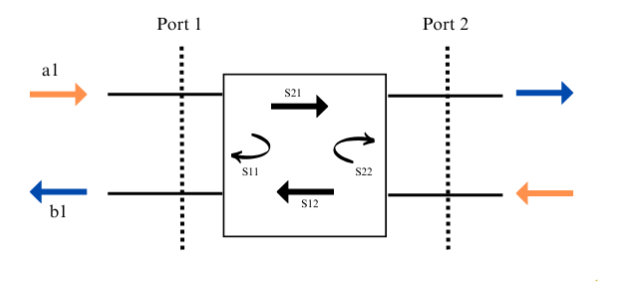
\includegraphics[width=0.7\textwidth]{Intro/device_2ports.png}
    \caption{Representation of the two-port device.}
    \label{fig:device_2ports}
\end{figure}

Let us define $a_i$ as the incident wave and $b_i$ as the reflected wave, with $i = 1,2$ representing port 1 and port 2, respectively. We can write the outgoing waves at the ports as:

$$
b_1 = S_{11}a_1 + S_{12}a_2
$$
$$b_2 = S_{21}a_1 + S_{22}a_2
$$

These relations can be expressed in matrix form, where $\mathbf{a}$ and $\mathbf{b}$ are vectors and the $S_{ij}$ terms are the coefficients of the so-called scattering matrix. 

\[
\begin{bmatrix}
b_1 \\
b_2
\end{bmatrix}
=
\begin{bmatrix}
S_{11} & S_{12} \\
S_{21} & S_{22}
\end{bmatrix}
\begin{bmatrix}
a_1 \\
a_2
\end{bmatrix}
\]

In particular, the index $i$ represents the output port, while $j$ represents the input port.

These values are defined as

\[
S_{ij} = \left.\frac{b_i}{a_j}\right|_{a_k=0,\;k\neq j}
\]

by setting to zero the contributions of the incident waves from all the other ports except the one being considered.


The diagonal terms, $S_{11}$ and $S_{22}$, represent the reflection coefficients of the respective ports, while the off-diagonal terms, $S_{21}$ and $S_{12}$, describe the transmission between the two ports.

\section{Measurement setup and calibration}
To set up the measurement environment, we used a Keysight VNA together with its dedicated software. First of all, we configured the plots of the S-parameters that would be observed during the measurements. In particular, we used two windows: the first displaying the $S_{11}$ and $S_{22}$ parameters, and the second displaying $S_{12}$ and $S_{21}$. Observing all four S-parameters allowed us to evaluate both the reflection and transmission behavior of the unknown device.\\
The frequency range for the entire laboratory session was set from 10 MHz to 6.5 GHz, with
a resolution of 1001 points uniformly distributed between the two edge values.\\
To minimize the effect of random noise during the measurements, we enabled a software setting that allows multiple acquisitions to be performed and then averaged in the displayed result. In our case, we used an average over 8 measurements.\\

Before starting the actual measurements, we performed the VNA calibration. The calibration procedure is important for removing systematic errors that may occur for several reasons, such as attenuation or phase shifts introduced by the cables connecting
the DUT to the VNA, as well as distortions caused by the internal couplers of the instrument.
To calibrate the VNA, we used an \textbf{Electronic Calibration kit} (E-cal kit), a device that is connected to the VNA and is able to emulate standards such as an open circuit, short circuit, precision load, and a through connection.
After connecting the E-Cal kit to the VNA, we started the calibration procedure through the software. This procedure consists of measuring the known standards emulated by the E-Cal kit and then using them as a reference to correct the measurements, thereby eliminating systematic errors.